\documentclass{notes}

\theoremstyle{plain}

\newtheorem{theorem}{Theorem}[chapter]
\newtheorem{definition}[theorem]{Definition}

\newcommand{\cO}{\mathcal{O}}
\newcommand{\cL}{\mathcal{L}}
\DeclareMathOperator{\sech}{sech}

\begin{document}
\frontmatter
\title{Methods}
\lecturer{Paul Metcalfe}
\maintainer{Paul Metcalfe}
\date{Summer 1998}
\maketitle

\thispagestyle{empty}
\noindent\verb$Revision: 1.8 $\hfill\\
\noindent\verb$Date: 1999/09/17 17:44:23 $\hfill\

\vspace{1.5in}

The following people have maintained these notes.

\begin{center}
\begin{tabular}{ r  l}
-- date & Paul Metcalfe
\end{tabular}
\end{center}

\tableofcontents

\chapter{Introduction}

These notes are based on the course ``Methods'' given by
Dr.~E.P.~Shellard in Cambridge in the Mich\ae lmas Term 1996.  These
typeset notes are totally unconnected with Dr.~Shellard.  They are
more vaguely based on the course than my notes usually are, and I have
mainly used Dr.~Shellard's notes to get a sense of ordering and
content.

\alsoavailable
\archimcopyright

\mainmatter

\chapter{Fourier series}

\section{Properties of sine and cosine}

Consider the set of functions
\[
g_n(x) = \cos \frac{n \pi x}{L} \qquad h_n(x) = \sin \frac{n \pi x}{L}
\]

with $n \in \N$.  These functions are periodic on $[0,2L]$ and are
also \emph{mutually orthogonal}:

\begin{align*}
\int_0^{2 L} \sin \frac{n \pi x}{L} \sin \frac{m \pi x}{L}\, \ud x
&= \begin{cases}
L \delta_{mn} & m, n \neq 0 \\
0 & m = n = 0.
\end{cases} \\
\int_0^{2L} \sin \frac{n \pi x}{L} \cos \frac{m \pi x}{L}\, \ud x & =
0 \\
\int_0^{2L} \cos \frac{n \pi x}{L} \cos \frac{m \pi x}{L}\, \ud x & =
\begin{cases}
L \delta_{m n} & m, n \neq 0 \\
2 L \delta_{0 n} & m = 0.
\end{cases}
\end{align*}

These properties are easy to verify by direct integration.

In fact the functions $g_n$, $h_n$ form a \emph{complete orthogonal
  set}; they span the space of functions periodic on $[0,2L]$.

\section{Definition of Fourier series}

We can expand any sufficiently well-behaved real periodic function
$f(x)$ with period $2L$ as

\begin{equation}\label{eq:fourdef}
f(x) = \frac{1}{2} a_0 + \sum_{n=1}^\infty a_n \cos \frac{\pi n x}{L}
+ \sum_{n=1}^\infty b_n \sin \frac{\pi n x}{L},
\end{equation}

where $a_n$ and $b_n$ are constants such that the series is convergent
for all $x$.  They are called \emph{Fourier coefficients} and can be
found using the results on orthogonality of $\sin$ and $\cos$:

\begin{align*}
\int_0^{2L} f(x) \sin \frac{m \pi x}{L}\, \ud x &= \sum_{n=1}^\infty
b_n \delta_{nm} = L b_m \\
\int_0^{2L} f(x) \cos \frac{m \pi x}{L}\, \ud x &= L a_m.
\end{align*}

Note that the $\frac{1}{2} a_0$ is \eqref{eq:fourdef} is not a typo,
but the $\frac{1}{2}$ is required for the above integral to work for
all $n$.  Note also that the particular interval used doesn't matter,
provided it is of length $2L$.

\subsubsection*{Example: sawtooth wave}\label{ref:sawtooth}

Define $f(x)$ by
\[
f(x) = x \qquad -L < x \le L
\] 

and let $f$ be periodic elsewhere.  We have

\[
a_n = \frac{1}{L} \int_{-L}^L x \cos \frac{n \pi x}{L}\, \ud x = 0
\quad \text{(odd function)},
\]

but

\[
b_n = \frac{2}{L} \int_0^L x \sin \frac{n \pi x}{L}\, \ud x
= \frac{2 L}{n \pi} (-1)^{n+1} \quad \text{(integrate by parts).} 
\]

Therefore the Fourier series is

\[
f(x) = \frac{2 L}{\pi} \left( \sin \frac{\pi x}{L} -
\frac{1}{2} \sin \frac{2 \pi x}{L} + \frac{1}{3} \sin \frac{3 \pi
  x}{L}
+ \dots \right).
\]

\begin{figure}
\begin{center}
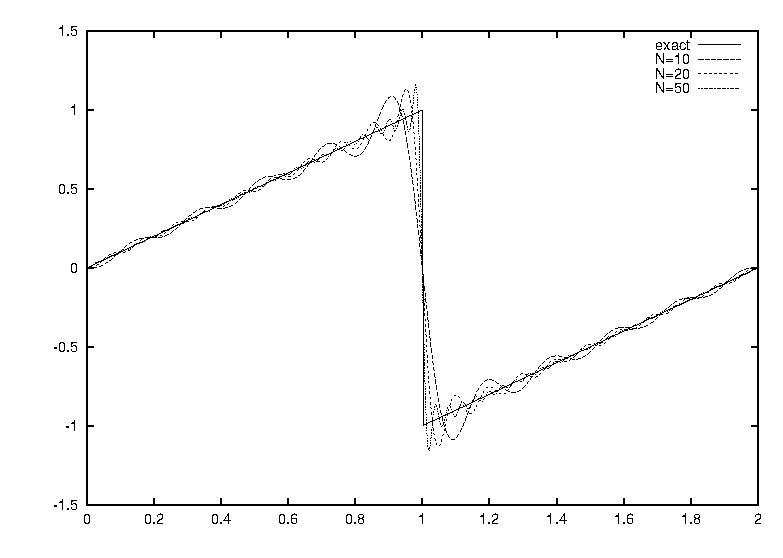
\includegraphics[scale=0.9]{sawtooth.eps}
\end{center}
\caption{Fourier series approximation showing Gibbs' phenomenon ($L = 1$)}%
\label{fig:sawtooth}
\end{figure}

We can plot the approximation
\[
f(x) \approx \frac{2 L}{\pi} \sum_{i=1}^N (-1)^{i+1} \sin \frac{i \pi x}{L}.
\]

This is shown in figure \ref{fig:sawtooth}.  We see that as $N$
increases the following occurs.

\begin{itemize}
\item The approximation improves away from the discontinuity --- it is
  convergent where $f$ is continuous.
\item The Fourier series tends to $0$ at $x=L$ --- the midpoint of the
  discontinuity.
\item The Fourier series has a persistent overshoot at $x=L$ of
  approximately $9 \%$ (Gibbs' phenomenon).
\end{itemize}

\subsection{The meaning of good behaviour}

The Dirichlet conditions are sufficiency conditions for a well-behaved
function $f(x)$ to have a convergent Fourier series.

\begin{theorem}
  If $f(x)$ is a bounded periodic function with period $2L$ with a
  finite number of maxima, minima and discontinuities in $[0,2L]$ then
  its Fourier series converges to $f(x)$ at all points where $f$ is
  continuous.  At discontinuities the series converges to the midpoint
  of the discontinuity: $\frac{1}{2} \left( f(x^-) + f(x^+)\right)$.
\end{theorem}

\begin{proof}
Omitted.
\end{proof}

Note that these are very weak conditions (compare Taylor's
theorem).  Pathological functions (e.g. $x^{-1}$, $\sin x^{-1}$) are
excluded.  The converse to this theorem is not true: $\sin
x^{-1}$ has a convergent Fourier series.

\section{Complex Fourier series}

It is obvious that we can rewrite \eqref{eq:fourdef} as

\[
f(x) = \sum_{n \in \Z} c_n e^{\frac{\imath n \pi x}{L}},
\]

where
\[
c_n = \frac{1}{2 L} \int_0^{2L} f(x) e^{-\frac{\imath n \pi x}{L}}\,
\ud x.
\]

This is sometimes useful (and also makes the analogy with Fourier
transforms slightly more obvious).

\section{Sine and cosine series}

Consider a function $f(x)$ defined only on the half interval $[0,L]$.
We can extend its range in two obvious ways by making it either odd or
even on $[-L,L]$.

If we make it odd then we put $a_n = 0$ and
\[
b_n = \frac{2}{L} \int_0^L f(x) \sin \frac{n \pi x}{L}\, \ud x
\]
in \eqref{eq:fourdef}.

If we make it even then $b_n = 0$ and

\[
a_n = \frac{2}{L} \int_0^L f(x) \cos \frac{n \pi x}{L}\, \ud x.
\]

\section{Parseval's theorem}

This is a relation between the average of the square of a function and
its Fourier coefficients.

\begin{align*}
  \int_0^{2 L} f(x)^2\, \ud x &= \int_0^{2 L} \left(\frac{1}{2} a_0 +
    \sum_{n=1}^\infty a_n \cos \frac{\pi n x}{L} + \sum_{n=1}^\infty
    b_n \sin \frac{\pi n x}{L} \right)^2 \, \ud x \\
  &= \int_0^{2 L} \left( \frac{1}{4} a_0^2
  + \sum_{n=1}^\infty a_n^2 \cos^2 \frac{\pi n x}{L} + \sum_{n=1}^\infty
    b_n^2 \sin^2 \frac{\pi n x}{L} \right)\, \ud x \\
  &= L \left(\frac{a_0^2}{2} +
    \sum_{n=1}^\infty \left(a_n^2 + b_n^2\right) \right).
\end{align*}

This is also called a \emph{completeness relation}.

\subsubsection*{Example: sawtooth wave}

Recall the sawtooth wave (page \pageref{ref:sawtooth}).  Here we had
$a_n = 0$ and $b_n = \frac{2 L}{n \pi} (-1)^{n+1}$.  Then applying
Parseval's relation gives

\[
\frac{2}{3} L^3 = \int_{-L}^L x^2\, \ud x =
L \sum_{n=1}^\infty \frac{4 L^2}{n^2 \pi^2},
\]

and so
\[
\sum_{n=1}^\infty n^{-2} = \frac{\pi^2}{6}.
\]

\chapter{The Wave Equation}

\section{Waves on an elastic string}

Consider small displacements on a stretched string with the endpoints
fixed and the initial conditions (displacement and velocity) given.

\vspace{1.5in}

Resolve horizontally to get
\[
T_1 \cos \theta_1 = T_2 \cos \theta_2.
\]

Now for small $\theta$, $\cos \theta \approx 1 - \frac{1}{2}
\theta^2$, and so $T_1 = T_2$ with error $\cO(\pd{y}{x})^2$.  

Resolving vertically,
\[
F_T = T_1 \sin \theta_1 + T_2 \sin \theta_2
= T \left( \left.\pd{y}{x}\right|_{x+\ud x} -
\left.\pd{y}{x}\right|_x \right) = T \pd{^2 y}{x^2} \ud x.
\]

Therefore (from Newton II)
\[
\mu \ud x\, \pd{^2 y}{t^2} = T \pd{^2 y}{x^2}\, \ud x,
\]

and so
\[
\pd{^2 y}{t^2} = \frac{T}{\mu} \pd{^2 y}{x^2}.
\]

This is the wave equation, with $c = \sqrt{\frac{T}{\mu}}$.   In
general, the 1D wave equation is

\begin{equation}\label{eq:1dwave}
\pd{^2 y}{t^2} = c^2 \pd{^2 y}{x^2}.
\end{equation}

\section{Separation of variables}

We want to solve \eqref{eq:1dwave} given the \emph{boundary
  values}

\[
y(0,t) = 0 \qquad y(L,t) = 0
\]

and the \emph{initial conditions}

\[
y(x,0) = p(x) \qquad \left.\pd{y}{t}\right|_{(x,0)} = q(x).
\]

We try a substitution $y = X(x) T(t)$ in \eqref{eq:1dwave}.  This
gives

\[
c^{-2} \frac{\Ddot{T}}{T} = \frac{X''}{X}.
\]

Since the LHS depends only on $t$ and the RHS only on $x$ they must
both be equal to a constant $\lambda$.

We have therefore split the PDE into two ODEs:

\[
X'' - \lambda X = 0 \qquad \text{and} \qquad \Ddot{T} - c^2 \lambda T
= 0.
\]

We solve the $x$ equation first:

\[
X'' - \lambda X = 0 \qquad X(0) = X(L) = 0.
\]

Since we don't know anything about $\lambda$ we have to learn
something...

\begin{itemize}
\item If $\lambda > 0$ the solution is $X = A \cosh \sqrt{\lambda} x
+ B \sinh \sqrt{\lambda} x$.  If we apply the boundary values now we
see that $A = B = 0$ --- so this is not a useful solution.
\item If $\lambda = 0$ the solution is $X = A + B x$, and as before
  $A=B=0$ on substituting the boundary values.
\end{itemize}

The only possibility now is $\lambda = - \nu^2$, which gives solutions

\[
X = A_\nu \cos \nu x + B_\nu \sin \nu x.
\]

Applying the boundary values gives $A = 0$ and $B_\nu \sin \nu L = 0$.
If $B_\nu = 0$ then the entire solution is trivial, so the only useful
solution has
\[
\sin \nu L = 0 \Rightarrow \nu = \frac{n \pi}{L} \Rightarrow
\lambda = - \frac{n^2 \pi^2}{L^2}.
\] 

These special values of $\lambda$ are \emph{eigenvalues} and their
\emph{eigenfunctions} are
\[
X_n = B_n \sin \frac{n \pi x}{L}.
\]

These are the \emph{normal modes}.  Now all we need to do is to solve
the $t$ equation using these values for $\lambda$:

\[
\Ddot{T} + \frac{n^2 \pi^2 c^2}{L^2} T = 0.
\]

This has a general solution
\[
T_n = C_n \cos \frac{n \pi c t}{L} + D_n \sin \frac{n \pi c t}{L}.
\]

Thus we have a \emph{specific solution} of \eqref{eq:1dwave}: $y_n =
T_n X_n$.  Since \eqref{eq:1dwave} is linear we can add solutions to
get the general solution

\begin{equation}\label{eq:1dwavesoln}
y(x,t) = \sum_{n=1}^\infty \left( C_n \cos \frac{n \pi c t}{L} + D_n
  \sin \frac{n \pi c t}{L} \right) \sin \frac{n \pi x}{L}.
\end{equation}

This satisfies the boundary values by construction.  The only
thing left to do is to satisfy the initial conditions:

\begin{align*}
y(x,0) &= p(x) = \sum_{n=1}^\infty C_n \sin \frac{n \pi x}{L} \\
\left.\pd{y}{t}\right|_{(x,0)} &= q(x)
= \sum_{n=1}^\infty \frac{D_n n \pi c}{L} \sin \frac{n \pi x}{L}.
\end{align*}

$C_n$ and $D_n$ can now be found using the orthogonality relations for
$\sin$.  They turn out to be

\[
C_n = \frac{2}{L} \int_0^L p(x) \sin \frac{n \pi x}{L}\, \ud x \qquad
D_n = \frac{2}{n \pi c} \int_0^L q(x) \sin \frac{n \pi x}{L}\, \ud x.
\]

\section{Oscillation energy}

A vibrating string has both KE and PE.  The KE is

\[
\frac{1}{2} \mu \int_0^L \Dot{y}^2\, \ud x
\]

and the PE is
\[
T \int_0^L \left(\sqrt{1 + y'{}^2} - 1 \right)\, \ud x
\approx \frac{1}{2} T \int_0^L y'{}^2\, \ud x.
\]

Since $c^2 = T \mu^{-1}$ the total sum is
\[
E = \frac{1}{2} \mu \int_0^L \Dot{y}^2 + \left( c y' \right)^2\, \ud x,
\]
which eventually evaluates as
\[
\frac{1}{4} \mu \sum_{n=1}^\infty \frac{n^2 \pi^2 c^2}{L^2}
\left(C_n^2 + D_n^2\right)
= \sum_{\text{normal modes}} \text{energy in mode.}
\]

The energy is conserved in time --- there is no dissipation.  Further,
there is no transfer of energy between modes.

\section{Solution in characteristic co-ordinates}

Consider the 1D wave equation \eqref{eq:1dwave}
\[
\pd{^2 y}{x^2} - c^{-2} \pd{^2 y}{t^2} = 0
\]

and make the change of variables $\xi = x + ct$, $\eta = x - ct$.
Using the chain rule this becomes
\[
4 \pd{^2 y}{\xi \partial \eta} = 0,
\]

with a general solution $y(\xi,\eta) = f(\xi) + g(\eta)$.  Thus the
general solution to \eqref{eq:1dwave} is

\[
y(x,t) = f(x+ct) + g(x-ct).
\]

This is a superposition of left and right moving waves.

Travelling waves (e.g. $g(x-ct)$) move with a constant speed $c$ and
retain their shape along characteristics (e.g. the line $x-ct = \text{const}$).

\section{Wave reflection and transmission}

Suppose there is a density discontinuity in the string, say at $x=0$.
This becomes a discontinuity in $c$ (although $T$ is a constant).  Let
\[
c = \begin{cases}
c_- & x < 0 \\
c_+ & x > 0.
\end{cases}
\]

\vspace{1.5in}

Consider a given harmonic incident wave
$A \exp\imath \omega \left(t - \frac{x}{c_-} \right)$. We want to find
the reflected wave $B \exp\imath \omega \left(t + \frac{x}{c_-}
\right)$ and the transmitted wave $C \exp\imath \omega \left(t - \frac{x}{c_+}
\right)$.

The string does not break at $x=0$, so that $y$ is continuous for all
$t$.  This gives $A+B=D$.

We further want the forces to balance at $x=0$:

\[
\left.T \pd{y}{x}\right|_{x=0^-} = \left.T \pd{y}{x}\right|_{x=0^+},
\]

and so $\pd{y}{x}$ is continuous for all time.  This condition gives
\[
- \frac{A}{c_-} + \frac{B}{c_-} = - \frac{D}{c_+}.
\]

We can now solve to find
\[
B = \frac{c_+ - c_-}{c_+ + c_-} A \qquad D = \frac{2 c_+}{c_+ + c_-} A.
\]

Note that the phase of the wave can (and generically does) change.

\chapter{Green's Functions}

\section{The Dirac delta function}

Define a generalised function $\delta(x-\xi)$ with the properties
$\delta(x-\xi) = 0$ for $x \neq \xi$ and
\[
\int_{-\infty}^\infty \delta(x-\xi)\, \ud x = 1.
\]

These two properties imply
\[
\int_{-\infty}^\infty f(x) \delta(x-\xi)\, \ud x = f(\xi).
\]

Note that

\begin{itemize}
\item $\delta$ is \emph{not} a function, but is classified as a
  distribution.\footnote{See PDE's IIB for more details (than you could
    possibly want).}
\item It is always employed in an integrand as a linear operator,
  where it is well defined.
\end{itemize}

\subsection{Representations}

We can represent the delta function as some sort of functional limit.
A discontinuous representation is

\[
\delta_\epsilon(x) = \begin{cases}
0 & x < - \frac{\epsilon}{2} \\
\epsilon^{-1} & - \frac{\epsilon}{2} \le x \le \frac{\epsilon}{2} \\
0 & x > \frac{\epsilon}{2},
\end{cases}
\]

and a continuous representation is

\[
\delta_\epsilon(x) = \frac{1}{\epsilon \sqrt{\pi}} e^{-\frac{x^2}{\epsilon^2}}.
\]

These are obviously both with $\epsilon \to 0$.  Examples with $n \to
\infty$ are
\[
\delta_n(x) = \frac{\sin n x}{\pi x} = \frac{1}{2 \pi} \int_{-n}^n
e^{\imath k x}\, \ud x
\]

and $\delta_n(x) = \frac{n}{2} \sech^2 n x$.

The Heaviside step function is

\[
H(x) = \begin{cases}
0 & x < 0 \\ 1 & x \ge 0,
\end{cases}
\]

and can be seen to be
\[
H(x) = \int_{-\infty}^x \delta(\xi)\, \ud \xi.
\]

Thus (in some suitably refined sense) $H'(x) = \delta(x)$.  We can also
define the derivative of the delta function such that we can integrate
it by parts:

\[
\int_{-\infty}^\infty f(x) \delta'(x - \xi)\, \ud x =
[ f(x) \delta(x-\xi) ]_{-\infty}^\infty - \int_{-\infty}^\infty f'(x)
\delta(x- \xi)\, \ud x = -f'(\xi).
\]

\section{Second order linear ODEs}

We wish to solve the general second order linear ODE:

\begin{equation}\label{eq:secord}
\cL y \equiv y'' + b(x) y' + c(x) y = f(x).
\end{equation}

We know that the homogeneous equation (with $f \equiv 0$) has two
linearly independent solutions $y_1$ and $y_2$, which give the
homogeneous equation the \emph{complementary function} solution $y_c
= A y_1 + B y_2$.  The inhomogeneous equation also has a particular
solution $y_p$.  The general solution of \eqref{eq:secord} is then
$y_c + y_p$.  Two boundary values (or initial conditions) are required
to find $A$ and $B$.

We hope to solve the boundary value problem.  We will restrict to
\emph{homogeneous} boundary values: $y(a) = y(b) = 0$.  More
general values can be turned into homogeneous ones by judicious use
of the complementary function.

\section{Definition of Green's function}

The Green's function $G(x,\xi)$ is the solution of
\[
\cL G(x,\xi) = \delta(x,\xi)
\]

with $G \equiv 0$ at endpoints.  By linearity we can now construct the
solution of \eqref{eq:secord} for general $f$:

\[
y(x) = \int f(\xi) G(x,\xi)\, \ud x.
\]

Now $y$ clearly satisfies the homogeneous boundary values, and it
is also easy to see that $\cL y = f$.

\subsection{Defining properties}

$G(x,\xi)$ splits into two halves

\[
G(x,\xi) = \begin{cases}
G_1(x,\xi) & a < x < \xi \\
G_2(x,\xi) & \xi < x < b.
\end{cases}
\]

such that $G$ solves the homogeneous equation for $x \neq \xi$, is
continuous at $x=\xi$ and satisfies $\left[G' \right]_{\xi^-}^{\xi^+}
= 1$.  Note that there are many different conventions for this jump
condition.

\section{Constructing $G(x,\xi)$: boundary value problems}

There is a solution to the homogeneous problem $y_-(x)$ such that
$y_-(a) = 0$.  Then $G_1(x,\xi) = C y_-(x)$.  Similarly there is a
solution $y_+(x)$ such that $y_+(b) = 0$ and so $G_1(x,\xi) = D y_+(x)$.
Now impose continuity at $x=\xi$ to give
\[
C y_-(\xi) = D y_+(\xi).
\]

The other equation comes from the jump condition:

\[
D y_+'(\xi) - C y_-'(\xi) = 1.
\]


We can solve these equations to give
\[
C = \frac{y_+(\xi)}{W(\xi)} \qquad D = \frac{y_-(\xi)}{W(\xi)},
\]
where $W(\xi)$ is the Wronskian:

\[
W(\xi) = y_-(\xi) y_+'(\xi) - y_+(\xi)y_-'(\xi).
\]

Thus

\[
G(x,\xi) = \begin{cases}
\frac{y_-(x) y_+(\xi)}{W(\xi)} & x < \xi \\
\frac{y_+(x) y_-(\xi)}{W(\xi)} & x > \xi,
\end{cases}
\]

and the solution of $\cL y = f$, $y(a) = y(b) = 0$ is

\[
y(x) = y_+(x) \int_a^x \frac{f(\xi) y_-(\xi)}{W(\xi)} \, \ud\xi +
y_-(x) \int_x^b \frac{f(\xi) y_+(\xi)}{W(\xi)}\, \ud\xi.
\]

\subsection{Derivation of jump conditions}

First suppose $G(x,\xi)$ is discontinuous at $x=\xi$, so that near
$x=\xi$,
\[
G(x,\xi) \propto H(x-\xi) \quad G'(x,\xi) \propto \delta(x-\xi) \quad
G''(x,\xi) \propto \delta'(x-\xi).
\]

Then the equation $\cL G = \delta(x-\xi)$ becomes

\[
\alpha \delta'(x-\xi) + \beta \delta(x-\xi) + \gamma H(x-\xi)
= \delta(x-\xi),
\]

which is certainly not possible.  So $G(x,\xi)$ is continuous at
$x=\xi$.  The jump condition in $G'$ can be derived by integrating
$\cL G = \delta(x-\xi)$ across $x = \xi$:

\[
\left[ G' \right]_{\xi^-}^{\xi^+} +
\underbrace{b(\xi) \left[ G \right]_{\xi^-}^{\xi^+}
+ \int_{\xi^-}^{\xi^+} (c-b') G\, \ud x}_{\to 0 \text{ as }
\xi^-,\xi^+ \to \xi} = 1.
\]

Therefore
\[
\left[ G' \right]_{\xi^-}^{\xi^+} = 1.
\]

\subsection{Example}

Suppose we wish to solve

\[
y'' = f(x) \qquad y(0) = y(L) = 0.
\]

The homogeneous solutions are $y = A x + B$ and so
$G_1 = C x$ and $G_2 = D (x - L)$.

Applying the continuity condition
\[
C \xi = D (\xi - L)
\]

and then the jump condition
\[
D - C = 1
\]

gives $D = \frac{\xi}{L}$ and $C = \frac{\xi -L}{L}$.

\section{Constructing $G(x,\xi)$: initial value problems}

Greens' function methods can also solve initial value problems.
Suppose we wish to solve $\cL y = f$, $y(0) = y'(0) = 0$.  Split $G$
into $G_1$ and $G_2$ as before.

Since $G_1(a) = G_1'(a) = 0$ and $\cL G_1 = 0$ then $G_1 \equiv 0$.
Therefore $G_2(\xi) = 0$ and $G_2'(\xi) = 0$, so that

\[
G(x,\xi) = \begin{cases}
0 & x < \xi \\
\frac{y(x)}{y'(\xi)} & x > \xi,
\end{cases}
\]

where $\cL(y) = 0$ and $y(\xi) = 0$.  The solution is then

\[
y(x) = y(x) \int_a^x \frac{f(\xi)}{y'(\xi)}\, \ud \xi.
\]

We see that causality is built in to the solution.

\subsection{Example}

Solve $y'' - y = f(x)$, $x > 0$, $y(0) = y'(0) = 0$.

In $x < \xi$, $G(x,\xi) = 0$ and in $x > \xi$ we have
\[
G(x,\xi) = A e^x + B e^{-x}.
\]

Continuity at $x = \xi$ gives $G(x,\xi) = C \sinh (x - \xi)$ in $x >
\xi$.  Now $y'(\xi) = C$ and so $C = 1$.  Hence

\[
y(x) = \int_0^x f(\xi) \sinh (x-\xi)\, \ud \xi.
\] 

\chapter{Sturm-Liouville Theory}

\section{Self-adjoint form and boundary values}

We wish to solve the general eigenvalue problem

\begin{equation}\label{eq:geneig}
\cL y = y'' + b(x) y' + c(x) y = - \lambda d(x) y
\end{equation}

with specified boundary conditions.  This often occurs after
separation of variables in a PDE.  One classic example is the
Schr\"odinger equation:

\[
\left(- \frac{\hbar^2}{2 m} \nabla^2 + V(\vect{x}) \right) \psi = \imath
  \hbar \pd{\psi}{t}.
\]

We try a solution $\psi = U(\vect{x}) e^{-\frac{\imath E t}{\hbar}}$.
Substituting into the Schr\"odinger equation gives
\[
\left(- \frac{\hbar^2}{2 m} \nabla^2 + V(\vect{x}) \right) U  = E U.
\]

$E$ is the energy eigenvalue.\footnote{See the Quantum Mechanics
  course for more details.}

The analysis greatly simplifies is $\cL$ is in \emph{self-adjoint
  form}: that is if \eqref{eq:geneig} can be re-expressed in
\emph{Sturm-Liouville form}:

\begin{equation}\label{eq:SLform}
\cL y = - (p y')' + q y = \lambda w y,
\end{equation}

where the \emph{weighting function} $w(x)$ is assumed positive.  We
can easily put \eqref{eq:geneig} in Sturm-Liouville form: multiply by
$\exp \int^x b(\xi)\, \ud\xi$.

\begin{definition}
$\cL$ is self-adjoint on the interval $a < x < b$ iff for all pairs of
functions $y_1$, $y_2$ satisfying appropriate boundary values we
have
\begin{equation}\label{eq:SAdefn}
\int_a^b y_1 \cL y_2\, \ud x = \int_a^b y_2 \cL y_1\, \ud x.
\end{equation}
\end{definition}

If we substitute \eqref{eq:SLform} into \eqref{eq:SAdefn} we see that
``appropriate boundary values'' means
\[
\left[ -y_1 p y_2' + y_2 p y_1' \right]_a^b = 0,
\]

which includes $y(a)=y(b)=0$, $y'(a) = y'(b) = 0$, $y +k y' = 0$,
$y(a) = y(b)$, $p(a) = p(b) = 0$ or combinations of the above.

\section{Eigenfunction expansions}

Self-adjoint operators have three important properties.

\subsection{Real eigenvalues}

Suppose $\cL y_n = \lambda_n y_n$, and so $\cL y_n^* = \lambda_n^*
y_n^*$.  Then

\[
\int_a^b y_n^* \lambda_n w y_n\, \ud x - \int_a^b \lambda_n^* y_n
y_n^*\, \ud x = 0
\]

and so $\lambda_n^* = \lambda_n$, since $\int w \abs{y_n}^2 \neq 0$
for non-trivial $w$, $y_n$.

\subsection{Orthogonal eigenfunctions}

Suppose $\lambda_m \neq \lambda_n$.  Then

\[
\left( \lambda_n - \lambda_m \right) \int_a^b w y_m y_n\, \ud x = 0
\]

and so $\int w y_m y_n = 0$.  $y_n$, $y_m$ are thus orthogonal on
$[a,b]$ wrt the weighting function $w(x)$.

\subsection{Complete eigenfunctions}

We can write sufficiently nice $f(x)$ as 

\[
f(x) = \sum_n a_n y_n(x),
\]

with

\[
\int_a^b f(x) y_n(x)\, \ud x = a_n \int_a^b w y_n^2\, \ud x.
\]

The eigenfunctions are sometimes normalised to unit modulus for convenience.

We also have Parseval's identity, which in this form is

\[
\int_a^b \left( f - \sum_{n=1}^\infty a_n y_n \right)^2 w\, \ud x = 0,
\]

or
\begin{equation}\label{eq:genPar}
\int_a^b w f^2\, \ud x = \sum_{n=1}^\infty \int_a^b w y_n^2\,\ud x.
\end{equation}

The expansions needed converge if the eigenfunctions are complete.  If
the eigenfunctions are not complete then the LHS of \eqref{eq:genPar}
is greater than its RHS.  This is \emph{Bessel's inequality}.

\section{Example: Legendre polynomials}

Consider Legendre's equation

\begin{equation}\label{eq:Legendre}
(1-x^2) y'' - 2 x y' + \lambda y = 0,
\end{equation}

which can be rewritten in Sturm-Liouville form as

\[
- \diff{}{x} \left( (1-x^2) y' \right) = \lambda y.
\]

It is motivated by separation of variables in spherical polars.  The
boundary conditions are that $y$ is finite at $x = \pm 1$.  We try a power
series solution about $x=0$,
\[
y = \sum_{n=0}^\infty c_n x^n,
\]

which gives (prove this)
\[
c_{n+2} = \frac{n(n+1) - \lambda}{(n+1)(n+2)} c_n.
\]

Specifying $c_0$ and $c_1$ yields linearly independent solutions, one
of which is odd and the other even.

As $n \to \infty$, $\frac{c_{n+2}}{c_n} \to 1$ and so we get a
geometric series, which is divergent at $x= \pm 1$.  One of the two
series must terminate and so $\lambda = m(m+1)$ for $m \in \N$.

The eigenfunctions on $-1 \le x \le 1$ are the \emph{Legendre
  polynomials} $P_n$.  $P_n$ is usually normalised so that $P_n(1) = 1$: with
  this normalisation we have

\begin{center}
\begin{tabular}{r | c | l}
$n$ & $\lambda$ & $P_n$ \\ \hline
$0$ & $0$ & $1$ \\
$1$ & $2$ & $x$ \\
$2$ & $6$ & $\tfrac{1}{2} ( 3 x^2 - 1)$ \\
$3$ & $12$ & $\tfrac{1}{2} (5 x^3 - 3 x)$
\end{tabular}
\end{center}

The orthogonality relation is
\[
\int_{-1}^1 P_n P_m\, \ud x = \frac{2}{2 n + 1} \delta_{mn}.
\]

\section{Inhomogeneous boundary value problem}

\[
(\cL - \mu w) y = f(x).
\]

Consider the above inhomogeneous ODE with homogeneous boundary values
and a fixed $\mu$ (not an eigenvalue).

Now we can expand $f(x)$ in terms of eigenfunctions of $\cL$:

\[
f(x) = w(x) \sum_{n=1}^\infty a_n y_n,
\]

where
\[
a_n = \int_a^b f y_n\, \ud x
\]

and the eigenfunctions are normalised to $\int y_n^2\, \ud x = 1$.  We
seek a solution
\[
f = \sum_n b_n y_n.
\]

Substituting we find $b_n (\lambda_n - \mu) = a_n$ (by orthogonality)
and so provided $\mu$ is not an eigenvalue,

\[
y = \sum_n \frac{a_n}{\lambda_n - \mu} y_n(x)
= \sum_n \frac{y_n(x)}{\lambda_n - \mu} \int_a^b f y_n\, \ud x'.
\]

If $\mu$ is an eigenvalue then this is a resonant frequency: the
amplitude grows without limit and there is no solution consistent with
the boundary values.

\chapter{Applications: Laplace's Equation}

We seek to solve

\begin{equation}\label{eq:Lapl}
\nabla^2 \phi = 0
\end{equation}

by the method of separation of variables.

$\phi$ can represent the electrostatic potential, gravitational
potential, heat and so on.  \eqref{eq:Lapl} is the homogeneous version
of the \emph{Poisson equation} $\nabla^2 \phi = \rho$.

Boundary values can be given on

\begin{itemize}
\item $\phi$ : Dirichlet boundary conditions
\item $\vect{n} \cdot \nabla \phi$ : von Neumann boundary conditions,
\end{itemize}

specified on a boundary surface in 3D, boundary curve in 2D or
endpoints in 1D.

\section{Cartesians}

In Cartesians, $\nabla^2 = \pd{^2}{x^2} + \pd{^2}{y^2} +
\pd{^2}{z^2}$.  We seek a solution $\phi = X(x) Y(y) Z(z)$ and get

\[
\frac{X''}{X} = - \frac{Y''}{Y} - \frac{Z''}{Z} = \lambda_l
\]

Similarly $\frac{Y''}{Y} = \lambda_m$ and $\frac{Z''}{Z} = \lambda_n$,
where $\lambda_l + \lambda_m + \lambda_n = 0$.  We can then find eigenfunction
solutions satisfying the given boundary values: $\phi_{lmn} = X_l
Y_m Z_n$, so that then the general solution is

\[
\phi = \sum_{lmn} c_{lmn} X_l Y_m Z_n.
\]

\subsection*{Example: heat conduction}

Solve the system

\begin{align*}
\nabla^2 \phi &= 0 \quad \text{in $z>0$} \\
\phi &= 0 \quad \text{$x=0,1$ or $y=0,1$} \\
\phi &= 1 \quad \text{at $z=0$} \\
\phi &\to 0 \quad \text{as $z \to \infty$.}
\end{align*}

This models heat conduction on a semi-infinite square bar.

We separate variables to get $X_n = \sin l \pi x$ and $Y_m = \sin m
\pi x$, with $\lambda_l = -l^2 \pi^2$ and $\lambda_m = - m^2 \pi^2$.
Then we have
\[
\frac{Z''}{Z} = \pi^2 (l^2 + m^2),
\]

and so $Z_{l,m} = e^{-\pi z \sqrt{l^2 + m^2}}$ (to satisfy the bc at
infinity).  Therefore

\[
\phi = \sum_{l,m} A_{l,m} \sin l \pi x \sin m \pi y\, e^{-\pi z
  \sqrt{l^2 + m^2}}.
\]

To find $A_{l,m}$ use the boundary condition at $z=0$:
\[
1 = \sum_{l,m} A_{l,m} \sin l \pi x \sin m \pi y.
\]

Now
\[
\int_0^1 \sin l \pi t \sin m \pi t \, \ud t
= \frac{1}{2} \delta_{lm}
\]

and so

\[
\int_0^1 \int_0^1 \sin l \pi x \sin m \pi y\, \ud x \ud y = \frac{A_{l,m}}{4}.
\]

Thus

\[
A_{l,m} = \begin{cases}
\frac{16}{\pi^2 l m} & l,m \text{ odd} \\
0 & \text{otherwise.}
\end{cases}
\]

Note that in this case we have \emph{degenerate eigenvalues}: both
$X_1 Y_2$ and $X_2 Y_1$ give the same constant in the $z$ equation.
Despite this, we can always choose orthogonal eigenfunctions.

\section{Plane polars}

In plane polars, Laplace's equation becomes

\begin{equation}\label{eq:LapPlane}
\frac{1}{r} \pd{}{r} \left(r \pd{\phi}{r} \right) + \frac{1}{r^2}
\pd{\phi}{r^2} = 0.
\end{equation}

We seek $\phi = R(r) \Theta(\theta)$, which gives
\[
\frac{r (r R')'}{R} = \lambda \qquad \frac{\Theta''}{\Theta} = -\lambda.
\]

Consider a drum surface with a distorted rim, with unit radius.  The
height of the surface is given by $\phi$ such that $\nabla^2 \phi = 0$
and $\phi(1,\theta) = f(\theta)$.

Now the $\theta$ equation is

\[
\Theta'' + \lambda \Theta = 0
\]

and since $\Theta$ must be periodic, $\lambda = n^2$ for $n \in \N$.

The solution to this equation is

\[
\Theta_n = a_n \cos n \theta + b_n \sin n \theta.
\]

If $n=0$ then the solution is $\Theta_0 = a_0 + b_0 \theta$ : $b_0 =
0$ from the periodic boundary conditions.

The $r$ equation is
\[
r (r R')' - n^2 R = 0,
\]

which has solutions $R = c_n r^n + d_n r^{-n}$.  Thus $d_n = 0$ to
keep the solution finite in $r < 1$.  When $n = 0$ the solution is
$c_0 + d_0 \log r$ and so $d_0 = 0$.  Thus

\[
\phi(r,\theta) = \frac{1}{2} a_0 + \sum_{n=1}^\infty \left( a_n \cos n
\theta + b_n \sin n \theta \right) r^n.
\]

$a_n$ and $b_n$ can be found using $\phi(1,\theta) = f(\theta)$.

\section{Spherical polars}

The Laplace equation becomes

\begin{equation}\label{eq:sphLap}
\frac{1}{r^2} \pd{}{r} \left(r^2 \pd{\Phi}{r} \right) +
\frac{1}{r^2} \pd{}{\theta}
\left( \sin \theta \pd{\Phi}{\theta} \right) +
\frac{1}{r^2 \sin^2 \theta} \pd{^2 \Phi}{\phi^2} = 0.
\end{equation}

We seek separable solution $R(r) \Theta(\theta) \psi(\phi)$ and
specialise to the axisymmetric case:  $\psi = 1$.  Then we have

\[
(r^2 R')' - \lambda R = 0 \qquad (\sin \theta \Theta')' + \lambda \sin
\theta = 0.
\]

Putting $x = \cos \theta$ in the $\theta$ equation gives

\[
\diff{}{x} \left( (1-x^2) \diff{\Theta}{x} \right) + \lambda \Theta = 0.
\]

This is Legendre's equation \eqref{eq:Legendre}, and so from the
earlier analysis we know $\lambda_n = n(n+1)$.  The radial equation
becomes

\[
(r^2 R')'  - n(n+1) R = 0,
\]

Trying a solution $r^m$ given $m=n$ or $m = -n-1$, so the
eigenfunction expansion of $\Phi$ is

\[
\Phi = \sum_n \left(A_n r^n + B_n r^{-n-1} \right) P_n(\cos \theta).
\]

$A_n$ and $B_n$ can be determined from boundary conditions on a
spherical surface.

\subsection[The full glory of spherical polars]%
{** The full glory of spherical polars **}

If we drop the assumption of axisymmetry things become more
complicated.  The azimuthal eigenfunctions are $\psi_m = e^{\imath m
  \phi}$ and the polar eigenfunctions $P_l^m(\cos \theta)$ satisfy the
\emph{associated Legendre equation}

\[
\diff{}{x} \left( (1-x^2) \diff{\Theta}{x} \right) + \left(
l (l+1) - \frac{m^2}{1-x^2}\right) \Theta = 0.
\]

We combine the azimuthal and polar eigenfunctions to get the
\emph{spherical harmonics}:

\[
Y_{lm}(\theta,\phi) = \sqrt{\frac{(2 l + 1)! (l-m)!}{4 \pi (l+m)!}}
P_l^m(\cos \theta) e^{\imath m \phi},
\]

for $-l \le m \le l$.  The radial equation is the same as before, giving

\[
R_{lm} = a_{lm} r^l + b_{lm} r^{-l-1}.
\]

\chapter{Calculus of Variations}

\section{The problem}

Suppose we wish to minimise

\begin{equation}\label{eq:CoVprob}
J[y] = \int_{x_1}^{x_2} F(x,y,y')\, \ud x
\end{equation}

over all functions $y$ such that $y(x_1) = y_1$ and $y(x_2) = y_2$.
This is clearly not just an ordinary calculus minimization, but
something slightly harder...

\section{Euler-Lagrange equations}

We will do this, as in ordinary minimization problems, by finding a
function such that the first order variation of $J$ is zero.  So,
suppose $y(x)$ is the answer and perturb it slightly to $y(x) + \delta
y(x)$, where $\delta y(x_1) = \delta y(x_2) = 0$.  Then

\[
\delta F = \pd{F}{y} \delta y + \pd{F}{y'} \delta y' + \text{ higher order.}
\]

Hence

\begin{align*}
\delta J &= \int_{x_1}^{x_2} \delta y \pd{F}{y} + \delta y'
\pd{F}{y'}\, \ud x \\
&= \int_{x_1}^{x_2} \delta y \left(\pd{F}{y} - \diff{}{x} \pd{F}{y'}
\right)\, \ud x +
\underbrace{\left[ \delta y \pd{F}{y'}\right]_{x_1}^{x_2}}_{ = 0}.
\end{align*}

Thus for the first order variation to be zero we require

\begin{equation}\label{eq:EuLag}
\pd{F}{y} = \diff{}{x} \pd{F}{y'},
\end{equation}

since $\delta y$ is arbitrary.  This is an \emph{Euler-Lagrange
  equation}.

One variant on this that is sometimes useful: \eqref{eq:EuLag} is
equivalent to

\begin{equation}\label{eq:EuLag2}
\diff{}{x} \left( F - y' \pd{F}{y'} \right) = \pd{F}{x}.
\end{equation}

To prove this note that $\diff{}{x} = \pd{}{x} + y' \pd{}{y} + y'' \pd{}{y'}$.

There are three special cases:

\begin{itemize}
\item $y'$ absent gives $\pd{F}{y} = 0$, which can be solved
  for $y$.
\item $y$ absent gives $\pd{F}{y'} = \text{const}$.
\item $x$ absent gives $F - y' \pd{F}{y'} = \text{const}$ (use
  \eqref{eq:EuLag2}).
\end{itemize}

\section{Examples}

\subsection*{Geodesics}

In Euclidean $\R^2$ we have a metric $\ud s^2 = \ud x^2 + \ud y^2$ and
we seek to minimise
\[
\int_{x_1}^{x_2} \ud s = \int_{x_1}^{x_2} \sqrt{1 + y'{}^2}\, \ud x.
\]

We can immediately apply the Euler-Lagrange equations, noting that $y$
is absent and so

\[
\frac{y'}{\sqrt{1 + y'{}^2}} = \text{const,}
\]

which reduces to $y' = \text{const}$ and so the geodesics in $\R^2$
are straight lines (which is reassuring, if nothing else).

You can do something similar on the sphere, with
\[
\ud s^2 = \ud \theta^2 + \sin^2 \theta \ud \phi^2
\]

and show that the geodesics are great circles.

\subsection*{Brachistochrone}

Consider a frictionless bead on a wire path $y(x)$ connecting two points
$A$ and $B$.  What path gives the shortest travel time from $A$ to
$B$?

Assume $A$ is at $y=0$.  The time of travel is then

\[
T[y] = \int_A^B \frac{\ud s}{V} = \int_A^B \frac{\ud s}{\sqrt{2 g y}} 
= \frac{1}{\sqrt{2 g}} \int_{x_1}^{x_2} \sqrt{\frac{1 + y'{}^2}{y}}\, \ud x.
\]

$x$ is absent and the Euler-Lagrange equations eventually give

\[
y (1 + y'{}^2) = \text{const,}
\]

or
\[
x = \pm \int \left(\frac{y}{c-y} \right)^{\frac{1}{2}} \, \ud y.
\]

The substitution $y= c \sin^2 \frac{\theta}{2} = \frac{c}{2} ( 1- \cos
\theta)$ makes this integral doable and gives
\[
x = \pm \frac{c}{2} (\theta - \sin \theta)^2.
\]

\section{Principle of Least Action}

The action of a system is given by

\[
S = \int \cL\, \ud t,
\]

where $\cL = \text{KE} - \text{PE}$.  Trajectories minimize the
action.  Now suppose that $\text{KE} = \frac{1}{2} m \Dot{x}^2$ and
$\text{PE} = V(x)$.   Then

\[
\cL = \frac{1}{2} m \Dot{x}^2 - V(x)
\]

and the Euler-Lagrange equations give
\[
\diff{}{t} \left( m \Dot{x} \right) = V',
\]
which ought to be familiar...

Since $t$ is absent, we know that $\cL - \Dot{x}\pd{\cL}{\Dot{x}}$ is
constant --- in fact it is the total energy.

Something similar is Fermat's principle, that light follows the path
of minimum time.

Least action principles are important all over physics --- see the
General Relativity and Electrodynamics courses for more examples.

\section{Generalisations}

The trick with all of these is just to make the variation and see what
happens, integrating by parts where necessary.

The generalisation to several dependent variables is easiest: extremise

\[
J[\vect{y}] = \int_{x_1}^{x_2} F(x,\vect{y}, \vect{y}')\, \ud x.
\]

Performing the variation gives
\[
\pd{F}{y_i} = \diff{}{x} \pd{F}{y_i'}.
\]

Generalisations to several dependent variables exist: but it's easiest
just to do the variation explicitly.

The same is true of generalisations to more derivatives in $F$ ---
just do the variation and integrate by parts.

\section{Integral constraints}

Suppose we wish to extremise $J = \int F(x,y,y')\, \ud x$ subject to
the constraint $K = \int G(x,y,y')\, \ud x$ constant.  This is done by
using Lagrange multipliers: extremising

\[
I = \int F(x,y,y') + \lambda G(x,y,y')\, \ud x.
\]

Examples are on the problem sheet.

\chapter{Cartesian Tensors in $\R^3$}

Summation convention is used throughout this chapter unless
explicitly stated otherwise.

\section{Tensors?}

A tensor is an object represented in a particular co-ordinate system
by a set of functions called components such that the components in a
new co-ordinate system are related to the components in the old
co-ordinates in a prescribed way.

We will consider only orthogonal co-ordinate systems, and restrict the
transformations to rotations and reflexions.  More general
transformations and co-ordinate systems are possible --- see the
General Relativity course for details.

Consider a vector $\vect{x}$ with components $x_i$ in a given
orthogonal basis:

\[
\vect{x} = x_i \vect{e}_i.
\]

Now consider new co-ordinates $\vect{e}_i'$, such that
\[
\vect{e}_i' = \left(\vect{e}_i' \cdot \vect{e}_j \right) \vect{e}_j,
\]

and denote $\vect{e}_i' \cdot \vect{e}_j \equiv l_{ij}$.  Now
\[
\delta_{ij} = \vect{e}_i' \cdot \vect{e}_j'
= \left(l_{ik} \vect{e}_k\right) \cdot \left( l_{jm} \vect{e}_m\right)
= l_{i k} l_{j m} \delta_{k m} = l_{i k} l_{j k}.
\]

Also,

\[
\vect{e}_i = (\vect{e}_i \cdot \vect{e}_p') \vect{e}_p' = l_{pi} \vect{e}_p',
\]

and so
\[
\vect{x} = x_i \vect{e}_i = x_i l_{pi} \vect{e}_p'.
\]

Hence $x_p' = x_i l_{pi}$.

\section{Transformation laws}

\begin{itemize}
\item \emph{Scalars} remain invariant under a co-ordinate
  transformation.  \emph{Scalars} are zero-rank tensors.

\item A \emph{vector} $\vect{A}$ is a set of three functions $A_i$
  given in a particular co-ordinate system with the transformation
  property
\[
A_p' = l_{pi} A_i,
\]
so that $A_j'$ is a vector in a co-ordinate system rotated by $L$.  A
vector is a $1^{\text{st}}$ rank tensor.

\item A second rank tensor comprises 9 functions $A_{ij}$ in a given
  co-ordinate system such that
\[
A_{pq}' = l_{ip} l_{jq} A_{ij}.
\]

\item An $n^{\text{th}}$ rank tensor comprises $3^n$ functions of
  position such that

\[
A_{p q \dots r}' = l_{pi} l_{qj} \dots l_{rk} A_{ij \dots k}.
\]
\end{itemize}

We can see that $0 \leftrightarrow 0$, which means that tensor
equations are preserved by change of co-ordinate system.  To see this,
suppose $A$ and $B$ are tensors with $A_{ij \dots k} = B_{ij \dots k}$
in one co-ordinate system.  Then $A - B$ is a tensor --- it's zero,
and so $A'_{p q \dots r} - B'_{p q \dots r} = 0$ and hence $A'_{p q \dots r}
= B'_{p q \dots r}$.  This is why tensors are so useful.

\section{Tensor algebra}

Proof of all of these is obvious --- just show that they obey the
transformation law.

\begin{itemize}
\item If $A$ is a $n^{\text{th}}$ rank tensor then so is $\lambda A$
  for scalar $\lambda$.
\item If $A$ and $B$ are $n^{\text{th}}$ rank tensors then so is $C =
  A + B$.
\item If $A$ is an $n^{\text{th}}$ rank tensor and $B$ is an
  $m^{\text{th}}$ rank tensor then the outer product defined by
\[
C_{i j \dots k a b \dots c} = A_{i j \dots k} B_{a b \dots c}
\]
is an $(n + m)^{\text{th}}$ rank tensor.
\item If $A_{i j k \dots l}$ is an $n^{\text{th}}$ rank tensor then
  the contraction $A_{i i k \dots l}$ is an $(n-2)^{\text{th}}$ rank tensor.
\end{itemize}

\section{Quotient Laws}

\begin{theorem}[Quotient Theorem]
  If the inner product of some quantity $A$ with an arbitrary vector
  $\vect{K}$ is an $n^{\text{th}}$ rank tensor then $A$ is an
  $(n+1)^{\text{th}}$ rank tensor.
\end{theorem}

\begin{proof}

We know
\[
A_{ij \dots k} K_i = B_{j \dots k}
\]

In a new co-ordinate system

\begin{align*}
B'_{q \dots r} &= A'_{pq \dots r} K'_p \\
               &= l_{q j} \dots l_{r k} B_{j \dots k} \\
               &= l_{q j} \dots l_{r k} A_{ij \dots k} K_i \\
               &= l_{q j} \dots l_{r k} A_{ij \dots k} l_{pi} K'_{p},
\end{align*}

and so, since $K$ is arbitrary, $A'_{pq \dots r} = l_{pi} l_{q j}
\dots l_{r k} A_{ij \dots k}$.
\end{proof}

This theorem generalises to any type of product --- inner, outer or a
mixture thereof.  The proof is as above.

This can be used to identify the transformation properties of physical
quantities, for instance in \emph{Ohm's law}
\[
J_i = \sigma_{ij} E_j,
\]
where $\vect{J}$ is the current vector and $\vect{E}$ the electric
field vector, then the conductivity $\sigma$ must be a tensor.

\section{Isotropic tensors}

Isotropic tensors are invariant under all co-ordinate transformations:

\[
A'_{p q \dots r} = l_{pi} l_{qj} \dots l_{rk} A_{ij \dots k} = A_{p q
  \dots r}.
\]

Scalars are clearly isotropic.  As for vectors, suppose $A_p' = l_{pi}
A_i = A_p$.  Then

\[
(l_{pi} - \delta_{pi}) A_i = 0
\]

for all $l_{pi}$, so $A_i = 0$.

\begin{theorem}
The most general isotropic second rank tensor in $\R^3$ is $\lambda
\delta_{ij}$.
\end{theorem}

\begin{proof}
$\lambda \delta_{ij}$ is clearly isotropic, so we must prove that it
the the most general isotropic second rank tensor in $\R^3$.

Let $A_{ij}$ be isotropic, so that
\[
A_{pq}' = l_{pi} l_{qj} A_{ij} = A_{pq}.
\]
Rotate by $90^\circ$ around the $z$-axis --- i.e. take
\[
L = \begin{pmatrix}
0 & 1 & 0 \\ -1 & 0 & 0 \\ 0 & 0 & 1
\end{pmatrix}
\]

and then compare components.  Do the same thing with the $y$ axis.
\end{proof}

\begin{theorem}
The only isotropic third rank tensor is the alternator
$\epsilon_{ijk}$  (or the product of a scalar with the alternator).
\end{theorem}

\begin{proof}
The same as before, more or less.
\end{proof}

\begin{theorem}
The most general isotropic fourth rank tensor is
\[
A_{ijkl} = \lambda \delta_{ij} \delta_{kl} + \mu \delta_{ik}
\delta_{jl} + \nu \delta_{il} \delta_{jk}.
\]
\end{theorem}

\subsection{Spherically symmetric integrals}

Consider

\[
A_{ij} = \int_{r < a} x_i x_j\, \ud V.
\]

It is clearly isotropic, so $A_{ij} = \lambda \delta_{ij}$.  Now
contract over $i$ and $j$ to get

\[
3 \lambda = \int_{r < a} r^2\, \ud V = \frac{4 \pi a^5}{5}.
\]

Therefore
\[
\int_{r < a} x_i x_j\, \ud V = \frac{4 \pi a^5}{15} \delta_{ij}.
\]

This is a surprisingly easy way of doing the above integral!

\section{Symmetric and antisymmetric tensors}

If $A_{i j \dots k} = A_{j i \dots k}$ then $A$ is said to be
\emph{symmetric} in $i$ and $j$.  If $A_{i j \dots k} = - A_{j i \dots k}$
then $A$ is \emph{antisymmetric} or \emph{skew symmetric} in $i$ and
$j$.

If this is true in one co-ordinate system then it is true in all
co-ordinate systems (exercise).

Any second rank tensor can be decomposed into the sum of an
symmetric tensor and an antisymmetric tensor:

\begin{equation}\label{eq:Tdecomp1}
T_{ij} = \frac{1}{2} ( T_{ij} + T_{ji}) + \frac{1}{2} (T_{ij} - T_{ji}).
\end{equation}

Symmetric second rank tensors can be diagonalised.

Antisymmetric second rank tensors in $\R^3$ have only three
independent components:

\[
A_{ij} = \begin{pmatrix}
0 & a & b \\
-a & 0 & c \\
-b & -c & 0
\end{pmatrix} = \epsilon_{ijk} v_k,
\]

where $v_k = (c,-b,a)$.  We can therefore continue the decomposition
in \eqref{eq:Tdecomp1} into
\[
T_{ij} = \frac{1}{3} T_{kk} \delta_{ij} + \epsilon_{ijk} v_k + \Tilde{S}_{ij},
\]

the sum of a scalar part, a vector part and an irreducible tensor
part.

\section{Physical Applications}

Tensors have a very wide range of physical applications.  The relevant
courses are:

\begin{itemize}
\item Dynamics, Principles of Dynamics: angular momentum tensor, moment of
  inertia tensor.
\item Fluid Dynamics 2, Waves in Fluid and Solid Media, Theoretical
  Geophysics: stress tensor, strain tensor.
\item General Relativity: metric tensor, Riemann tensor, Ricci tensor.
\item Electrodynamics: Electromagnetic field tensor, stress-energy tensor.
\end{itemize}

\backmatter

\begin{thebibliography}{9}

\bibitem{Arfken} Arfken and Weber, \emph{Mathematical Methods for
    Physicists}, Fourth ed., Academic Press, 1995.
  
  {\sffamily \small Quite a lot of people sing Arfken's praises; I am
    not one of them.  Although it is useful I think it tries to do too
    much.  If nothing else though it could be used to kill small
    mammals and it does have everything in this course in it.  A good
    book to buy if you only want to buy one book in the next two
    years.  Or if you have a problem with mice. }
 
\end{thebibliography}

\section*{Related courses}

Most of the applied courses over the next two years use this course to
some extent.  You have been warned!

\end{document}